\documentclass[twocolumn]{article}
\usepackage[spanish]{babel}
\usepackage[utf8]{inputenc}
\usepackage[T1]{fontenc}
\usepackage{cite}
\usepackage{graphicx} 
\usepackage{float}
\usepackage{setspace}
\usepackage[font=small, skip=0pt]{caption}
\usepackage{enumitem} 
\begin{document}

\twocolumn[
\begin{center}
{\Large \textbf{Comparación de métodos de clasificación estadísticos con redes neuronales en la clasificación de imágenes de café tostado: sin tostar, ligero, medio y oscuro}}
\vspace{1ex}

Introducción a la Ciencia de Datos

Departamento de Ciencias de la Computación, CICESE

Francisco Regalado

Fecha: \today
\end{center}
\vspace{2ex}
\begin{center}
\textbf{Resumen}
\end{center}

\begin{quote}
En este proyecto se campara métodos de clasificación estadísticos y redes neuronales con la tarea de clasificar imágenes de granos de café tostado en cuatro niveles: sin tostar, tostado ligero, medio y oscuro, utilizando una base de datos de 1600 imágenes. Se evaluaron métodos estadísticos como Support Vector Classifier (SVC), Random Forest, Árbol de Decisión y K-Nearest Neighnors (KNN) aplicando técnicas de extracción de características como Análisis de Componentes Principales (PCA) y Histogramas de Gradientes Orientados (HOG), también se implementaron redes neuronales convolucionales VGGNet y DenseNet. Los resultados muestran que SVC con PCA alcanzo una precisión del 0.96, siendo el mejor entre los métodos de estadísticos, mientras que las redes neuronales lograron una precisión del 0.99 pero con un costo computacional significativamente mayor, con tiempos de entrenamiento de hasta 36 minutos frente a 1 minuto para SVC. Aunque las redes neuronales ofrecen mayor precisión, métodos estadísticos como SVC con PCA representan alternativas eficientes en términos de tiempo y recursos computacionales.
\end{quote}

\vspace{2ex}

]

\section{Introducción}

El consumo de café ha formado parte de la historia de la humanidad. El café ha sido más que un simple estimulante para despertar en las mañanas, también es un motor social y económico  \cite{uno}. El café ha evolucionado y recorrido un camino a lo largo del mundo. Resultado de esta adaptabilidad, ofrece un amplio espectro de sabores, debido a las grandes variaciones en el cultivo de las plantas y el proceso de extracción y procesamiento de los granos de café.

Uno de los factores que más contribuyen al sabor del café es el tipo de tostado al que se someten los granos. El tostado es muy importante, ya que el calor transforma la química interna del grano, desencadenando reacciones como la caramelización y la creación de compuestos volatiles que definen el aroma y el sabor \cite{dos}. Los diferentes niveles de tostado, que van desde los más claros hasta los oscuros, ofrecen distintos perfiles de sabor: desde notas brillantes y afrutadas hasta amargas y achocolatadas, incluyendo todo lo que esta en medio. Esta diversidad permite que cada consumidor encuentre un perfil que armonice con sus propias preferencias personales.

La clasificación de imágenes de granos de café tostados es una tarea que se puede abordar mediante métodos de clasificación en Python. La clasificación es una herramienta para segmentar automáticamente los datos en clases o categorías con características comunes. Estos, mediante el uso de algoritmos matemáticos, infieren patrones y relaciones existentes en el conjunto de datos, y luego usan el conjunto de entrenamiento para aprender y asignar etiquetas a nuevas observaciones. Más avanzados y potentes son aún lo métodos de redes neuronales. La capacidad de reconocer estructuras complejas en datos de alta dimensión es posible gracias a este tipo de redes. Las redes neuronales pueden aprender características jerárquicas y abstraer información relevante para la clasificación mediante múltiples capas de procesamiento, lo que proporciona una mayor precisión.

Resulta interesante contar con un método de clasificación efectivo para distinguir y categorizar con precisión los diferentes niveles de tostado, pues no existe un perfil de tostado superior a otro, si no que cada uno presenta características únicas que se adaptan a las necesidades y preferencias del consumidor. Un sistema de clasificación eficiente puede maximizar la calidad y consistencia de este producto, mejorando la cadena de suministro.


\section{Metodología}
La base de datos consiste en imágenes de granos de cafe tostado. Estos tostados están clasificados en tostado Bajo, Medio, Oscuro y sin tostar. La base de datos se divide en 4 clases, estas cuatro clases indican el nivel de tostado de los granos de café.

Existen 400 imagenes por clase, dando un total de 1600 imagenes con un tamaño de 224x224.
\begin{figure}[H] 
  \centering
  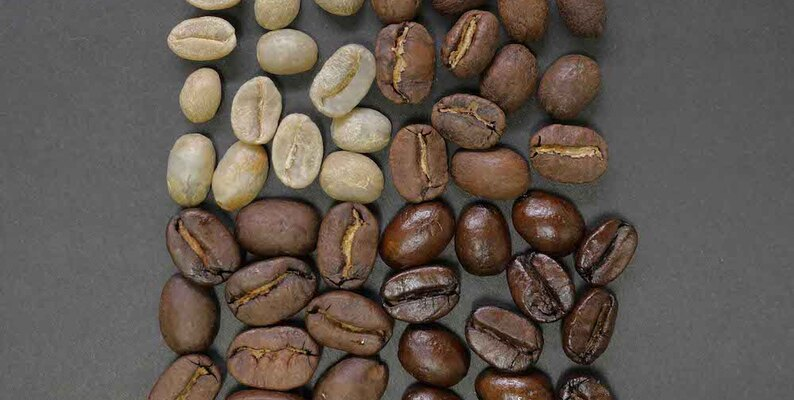
\includegraphics[width=0.8\columnwidth]{COVER.jpg} 
  \caption{Ejemplo de grano de las imágenes de las distintas clases.}
  \label{fig:verde} 
\end{figure}
La base de datos fue extraida de [Kaggle] \cite{tres}. 

Para realizar este proyecto se utilizarón 4 modelos de clasificación estadísticos: 
\begin{enumerate}[itemsep=0pt, parsep=0pt, leftmargin=*]
  \item \textbf{Support Vector Classifier}: Busca un hiperplano óptimo que separe las clases con el mayor margen posible.
  \item \textbf{Random Forest}: Combina múltiples árboles de decisión aleatorios para mejorar precisión y reducir sobreajuste.
  \item \textbf{Árbol de Decisión}: Divide los datos en subconjuntos basados en características, formando una estructura de árbol.
  \item \textbf{KNN}: Clasifica un dato asignándole la clase más común entre sus K vecinos más cercanos.
\end{enumerate}
 Fueron entrenados dos veces, primero utilizando PCA (Análisis de Componentes Principales) y luego con HOG (Histograma de Gradientes Orientados) para evaluar con que tipo de extracción de características estos métodos obtienen mejores resultados.
 
 Por otro lado, se implementaron 2 modelos de redes neuronales convolucionales:
 \begin{enumerate}[itemsep=0pt, parsep=0pt, leftmargin=*]
  \item \textbf{VGGNet}: Este modelo se compone de múltiples capas convolucionales seguidas por capas de agrupamiento y luego capas completamente conectadas. Se caracteriza por su simplicidad, ya que utiliza pequeñas ventanas de convolución y se profundiza al agregar muchas capas, lo que permite aprender representaciones jerárquicas más complejas.
  \item \textbf{DenseNet}: DeseNet conecta cada capa a todas las capas anteriores mediate conexiones de paso directo. Esto significa que cada capa recibe la entrada de todas las capas previas, lo que mejora el flujo de gradientes, fomenta la reutilización de características y permite usar menos parámetros.
\end{enumerate}
\section{Resultados}
A continuación, se presentan los resultados del proyecto.
\begin{figure}[H] 
  \centering
  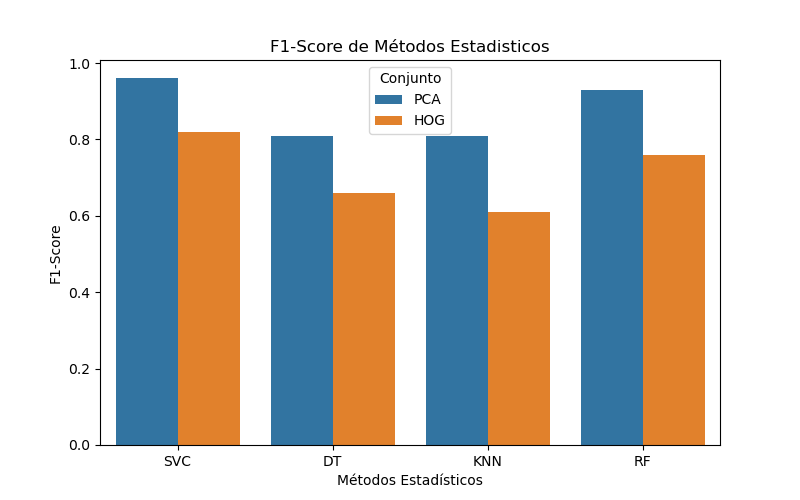
\includegraphics[width=0.97\columnwidth]{F1Colectiva.png} 
  \caption{F1-Score para cada método estadístico. Podemos observar como SVC y Random Forest sobresalen de KNN y Decision Tree (DT). }
  \label{fig:f1score} 
\end{figure}
\vspace{-25pt}
\begin{figure}[H] 
  \centering
  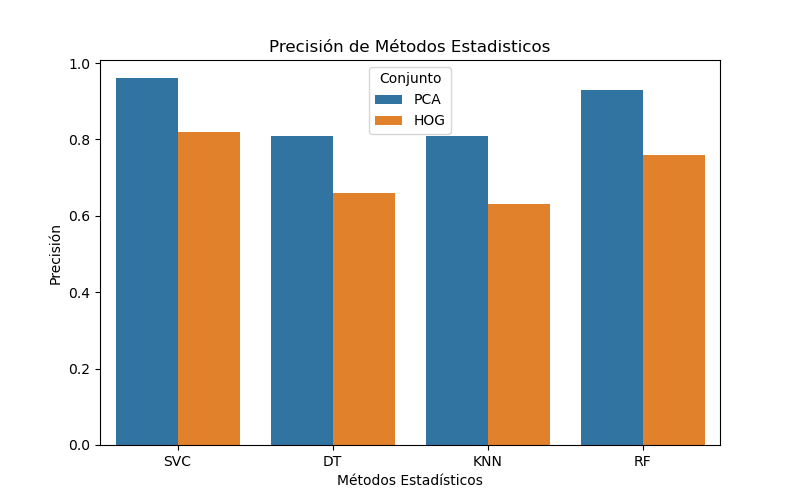
\includegraphics[width=0.97\columnwidth]{PrecisionColectiva.png} 
  \caption{Precisión para cada método estadístico. Podemos observar como SVC y Random Forest sobresalen de KNN y Decision Tree (DT). }
  \label{fig:precision} 
\end{figure}
\vspace{-25pt}
\begin{figure}[H] 
  \centering
  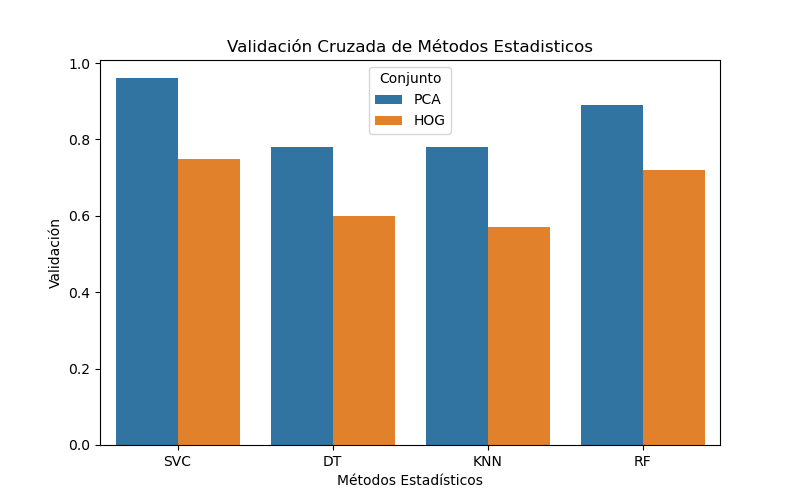
\includegraphics[width=0.97\columnwidth]{ValColectiva.png} 
  \caption{Validación Cruzada para cada método estadístico. En general, la validación cruzada es más robusta en PCA que utilizando HOG. }
  \label{fig:val} 
\end{figure}
\vspace{-16pt}

Para las redes neuronales, los resultados fueron de una precisión y F1-Score del 0.99 para ambos. Se utilizaron 50 épocas para cada red y así se obtuvieron las siguientes matrices de confusión:
\begin{figure}[H] 
  \centering
  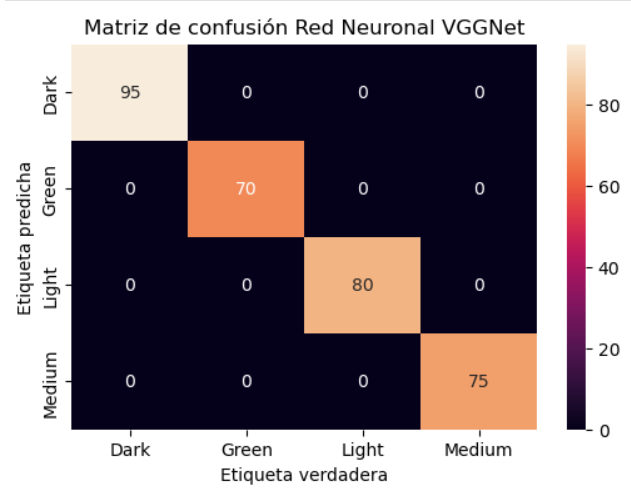
\includegraphics[width=0.8\columnwidth]{VGGNet.png} 
  \caption{Matriz de confusión para VGGNet.}
  \label{fig:Pvgg} 
\end{figure}
\vspace{-10pt}
\begin{figure}[H] 
  \centering
  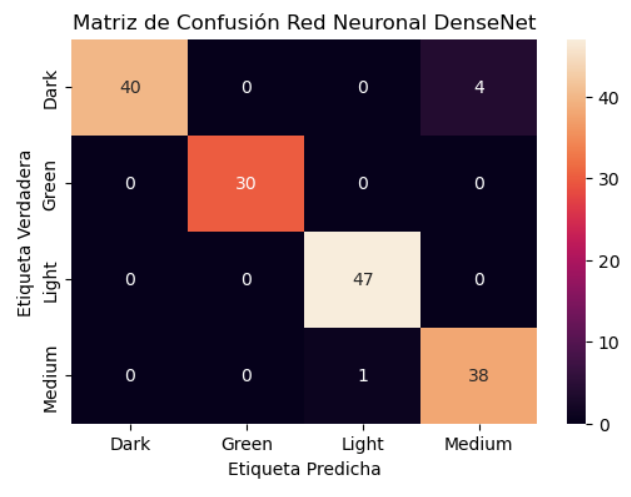
\includegraphics[width=0.8\columnwidth]{DenseNet.png} 
  \caption{Matriz de confusión para DenseNet.}
  \label{fig:PDN} 
\end{figure}
\vspace{-10pt}
Anexando la matriz de confusión para SVC con PCA, pues fue el método estadístico con mejores resultados.
\begin{figure}[H] 
  \centering
  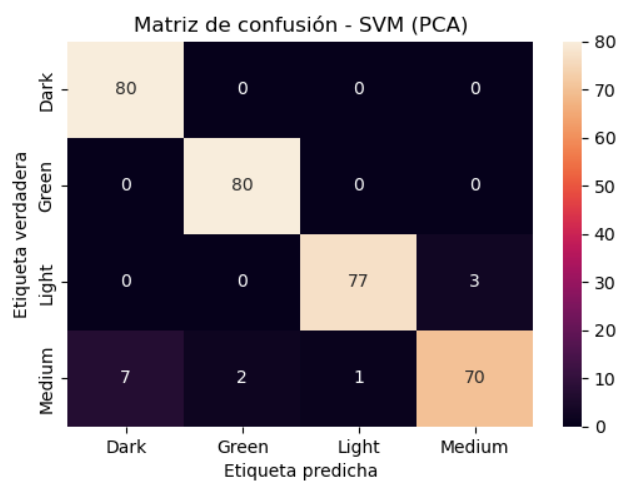
\includegraphics[width=0.8\columnwidth]{SVC(PCA).png} 
  \caption{Matriz de confusión para SVC utilizando PCA.}
  \label{fig:PSVC} 
\end{figure}
\vspace{-10pt}

\section{Discusión}

En los métodos estadísticos, utilizar PCA muestra mejores resultados que trabajar con HOG.
PCA es una técnica que reduce la dimensionalidad de los datos al identificar las direcciones (componentes principales) que capturan la mayor varianza en el conjunto de datos. En este contexto de imágenes de café tostado, las diferencias entre las clases Oscuro, Verde, Claro y Medio, probablemente en variaciones globales de color y textura. PCA puede ser efectivo para capturar estas variaciones globales, ya que considera la información de todos los pixeles y puede rescatar diferencias sutiles en tonalidad y luminosidad. 

HOG se enfoca en capturar características locales relacionadas con la forma y los bordes en una imagen, analizando las orientaciones de los gradientes en pequeñas regiones. Sin embargo, en las imágenes de granos de café tostado las diferencias entre las clases no restan realmente representadas por bordes o formas distintivas, si no más bien por patrones de color y texturas. Además, HOG convierte las imágenes en escala de grises perdiendo información importante para la clasificación.

Para estos métodos, SVC obtuvo el mayor rendimiento. Con un F1-Score de 0.96 y Precisión de 0.96 con una validación cruzada de 0.96 utilizando PCA. Mientras que, utilizando HOG, SVC obtuvo un F1-Score de 0.82 y Precisión de 0.76 con una validación cruzada de 0.72. Por lo que SVC usando PCA es el método con mejores resultados de los clasificadores estadísticos.

En comparación, las Redes Neuronales demostraron un rendimiento superior en tanto F1-Score y Precisión respecto a los métodos estadísticos. VGGNet, en su ultima época alcanzo un 0.99 de precisión y 0.99 de F1-Score. DenseNet obtiene números cercanos en su ejecución. VGGNet resulta ligeramente mejor que DenseNet en general. Ambas demuestran un rendimiento muy alto clasificando las imágenes. 

Evaluando los tiempos de ejecución en los métodos estadísticos con PCA, estos no pasaron de 2 minutos en la ejecución de los 4 modelos conjuntos. Utilizando HOG, la ejecución de los 4 modelos conjuntos alcanzo los 10 minutos, sin embargo no estuvo ni cercano a los resultados obtenidos mediante PCA. Pero estos quedan muy por atrás en cuando costo computacional utilizado por las redes neuronales. Para ambas los tiempos de ejecución fueron mayores de 20 minutos para este conjunto de entrenamiento a 50 épocas cada una. En promedio, el tiempo de entrenamiento fue de 25 minutos para DenseNet y 36 minutos para VGGNet.
 
El tiempo computacional se reduciría, disminuyendo la cantidad de épocas. Según las gráficas parece ser suficiente con 20 épocas, lo que reduciría el tiempo de entrenamiento para las redes neuronales. Aún teniendo esto en cuenta, el costo computacional sigue siendo mucho menor en los métodos estadísticos.

\section{Conclusión}

El método estadistico SVC utilizando Análisis de Componentes Principales (PCA) demostró ser muy eficiente para la clasificación de imágenes de café tostado, pues las métricos que logro (una precisión de 0.96) son cercanas a la de los modelos de Redes Neuronales (0.99) pero con un tiempo de entrenamiento mucho menor (1 minutos para SVC y 36 minutos para VGGNet). En el contexto en donde se necesite una alta precisión y no sea una limitante los recursos computacionales, las redes neuronales ofrecen un rendimiento adicional por su robustez de entrenamiento.


\begin{thebibliography}{9}

  
  \bibitem{uno}
  William Gervase Clarance-Smith,
  \emph{The Global Coffee Economy in Africa, Asia and Latin America, 1500-1989},
  Cambridge University Press, United Kingdom,
  1st Edition,
  2003.
  \bibitem{dos}
  Stefan Shenker, Trish Rothgeb,
  \emph{Chapter 11 -The Roast—Creating the Beans' Signature,},
  The Craft and Science of Coffee, Academic Press,
  Pag. 245-271,
  2017.
  
 \bibitem{tres}
 Gerry, Sroison, Sadipat, Thitaree,
\emph{Coffee Roast Intelligence},
Kaggle,
2017.
url:https://www.kaggle.com/datasets/gpiosenka/coffee-bean-dataset-resized-224-x-224/data

\end{thebibliography}


\end{document}